%\documentclass[smallroyalvopaper,twoside,12pt]{memoir}  % stocksize 9.25 by 6.175 in
\documentclass[a4paper,twoside,12pt]{memoir}  % stocksize A4
\usepackage{lipsum,amsmath,systeme}
\usepackage{graphicx}
\usepackage{mathtools}
%\usepackage{showframe}
\settrimmedsize{9in}{6in}{*} % final page size after trimming
\setulmarginsandblock{1in}{1in}{*} % upper and lower margins defining typeblock height
% according to KDP width of typeblock no more than 5.375in 
% about 65 characters per line is good for reading. For many 12pt fonts
% this gives a line length of about 2.5 alphabet lengths as about 5.2in.
% For 10pt fonts the line length is about 4.5in. Lets say the line length
% is to be 5in which calls for a 0.625in outer margin.
\setlrmarginsandblock{0.375in}{0.625in}{*}

\checkandfixthelayout

\begin{document}
\section{What is Linear Algebra?}
You've probably done algebra before in your life.
You've taken an equation like $x + 2 = 5$ and solved it to determine that
the only value of $x$ that makes it true is $x = 3$.

There are some equations that have no solutions, like $x + 1 = x + 2$.
There are also some equations that have more than one solution, like $x^2 = 4$.
In that equation, both $x = -2$ and $x = 2$ work.

Equations can have more than one variable.
For example, if I were to ask you ``Suppose I have two numbers that add up to six'', I would be asking you
to solve the equation $x + y = 6$. (There's many solutions to this: 0 and 6, 1 and 5, 3.5 and 2.5, etc.).

When there is more than one variable, we can draw pretty graphs.
Compare what these two graphs look like: (remember, the graph of an equation is just all the points that satisfy the equation)

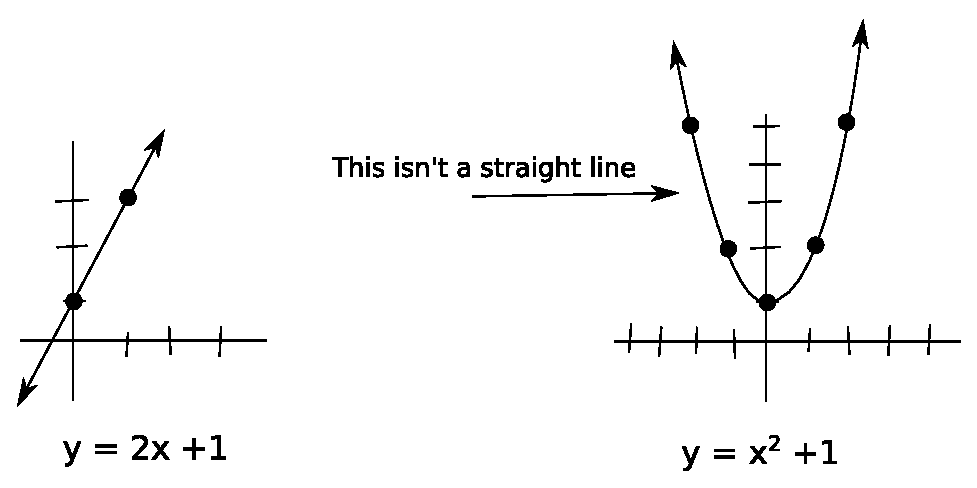
\includegraphics[width=\linewidth]{linear-vs-nonlinear.eps}

There's a difference between these two equations -- one is a straight line, the other is curvy.
(To be precise, $y = x^2 + 1$ is a parabola).

In linear algebra, we only deal with linear equations.
We don't deal with equations that make parabolas or orther curves\footnote{I should note that many time when a math book uses the word ``curve'' it includes straight lines, since a straight line is a just a curve that doesn't bend at all. When I use the word curve here I mean to exclude straight lines and to only mean things that are, you know, \ldots\ curvy.}.

How can you tell which equation will be a straight line? The exponent on the variables give it away. If the exponent is a one or a zero\footnote{Quick reminder about exponents of zero: $a^0$ will always be $1$, for any value of $a$. One reason why it is this way is to look at the pattern $3^1 = 3, 3^2 = 9, 3^3 = 27$. Every time we increase the exponent, we multiply be $3$. Going the other way, we \textit{divide} by $3$, so $3^0 = \frac{3}{3} = 1$. Another reason is that otherwise the exponent rules would break: $x^{a+b} = x^a*x^b$ means that $5^2 = 5^{2+0} = 5^2*5^0$. Therefore $5^0$ must be 1.} it will be straight. If any variable has an exponent besides one or zero it will be curvy.

Examples:
\begin{list}{}
\item $x + 2 = 4$ is a linear equation.
\item $x^2 + 2 = 4$ is not a linear equation.
\item $x + y + z = 3$ is a linear equation.
\item $x + y^{1.1} + z = 3$ is not a linear equation.
\end{list}

There's one more thing that can cause an equation to be non-linear: if it contains a non-linear function, then the equation will also be non-linear. Consider the sine function:

\includegraphics[height=1.5in]{sine_isnt_linear.eps}

That's not straight at all! Therefore, an equation like $5 \sin(x) = 5$ is non-linear.

Now, it may seem like there's no fun in linear algebra -- you probably already know how to solve an equation like $x + 2 = 4$, so where's the challenge?
In linear algebra, so solve \textit{multiple equations at once}.

For example, if I told you ``the sum of two numbers is 5, and their difference is 1, what are the numbers?'' you would want to be able to determine that the numbers are $3$ and $2$.

I could write that same problem as
\begin{equation*}
  \systeme{
    x + y = 5,
    x - y = 1
    }
\end{equation*}
We would say that $x = 3, y = 2$ \textit{solves the system} since it works for both of the equations.
(The little thing to the left of the equation is called a ``curly brace'' and is used to indicated that both of the equations are grouped together into a system.)

In the remainder of this chapter, we'll be learning how to solve linear systems of any size.
Then we'll go on to see what shapes linear systems represent, and some really cool and mysterious tie-ins with the rest of mathematics.

\subsection{Exercises}
Which of the following are linear equations?
\begin{list}{}
\item 1) $3 - x = 2$
\item 2) $3 + 4 -5 + x = 0$?
\item 3) $5 = 5$
\item 4) $0 = 5$
\item 5) $x + y = 2$
\item 6) $x^2 + y = 2$
\item 7) $5x + \cos(x) = 10$
\end{list}

\section{History of Linear Algebra}
%TODO

\section{Adding Equations Together}
Before we jump into solving systems of linear equations, we need to talk about one neat little trick: you can add equations together.

With an equation, the left-hand side equals the right-hand side. Since each side contains the same quantity, adding the same quantity to both sides of an equation will give you another equation which is also true.
Example: adding $5$ to each side of $x - 5 = 2$ gives us $x - 5 + 5 = 2 + 5$ and therefore $x = 7$.

Now consider $x + y = 5$ and $x - y = 1$. We can add $1$ to each side of $x + y =5$: $x + y + 1 = 5 + 1$.
But since the second equation says that $x - y = 1$, we can do a substitution: $x + y + (x - y) = 5 + 1$.

%TODO make a pretty picture of this.

Now that we know it's okay to add two equations together, it's easiest to just line everything up like below and add them together:

%TODO make and example of the equation

This gave us $2x = 6$, so $x = 3$. Using that information it would be eay to plug in $3$ for $x$ and determine what $y$ should be.

Examples:
\begin{list}{}
\item Adding $x + y = 4$ to $-x + y = 2$ gives $2y = 6$ (which simplifies to $y=3$.
\item Adding $x = 2$ to $y=3$ gives $x + y = 5$.
\item Adding $2x = 4$ to $-x = -2$ gives $x = 2$.
\end{list}

\subsection{Exercises}
\subsubsection{Add each pair of equations together.}

\begin{list}{}
\item 1) $x + y = 3$ and $x - y = 2$.
\item 2) $x + y + z = 4$ and $x - y - z = 8$.
\item 3) $x = 1$ and $x = 1$. (Don't forget to simplify).
\item 4) $x = 1$ and $-x = -1$.
\end{list}

\subsubsection{Which of the following is a linear equation?}
\begin{list}{}
\item 5) $x + y^2 = 5$
\item 6) $x - y  + z= 2$
\end{list}

\section{Systems and Solutions}
A few pages ago we saw the following system of equations:
\begin{equation*}
  \systeme{
    x + y = 5,
    x - y = 1
    }
\end{equation*}

A \textit{system} of equations is simply a group of equations where we'd like to find values for our variables that work for all of the equations in the system.

For example, $x=4, y=1$ works as a solution for $x+y=5$, since $4+1=5$, but it does not work as a solution for $x-y=1$, since $1-4 = -3 \neq 1$. Likewise, $x=100, y=99$ works as a solution for $x-y=1$, but not for $x+y=5$. However, $x=3,y=2$ works in both equations, so we say that $x=3, y=2$ is a solution of the system.

Sometimes in math we get fancy and say that $x=3, y=2$ is in the \textit{solution set} of the system.
That's just a fun way of saying that it's a solution to the system\footnote{Why say that there's a solution set? Because some systems have more than one solution.}.
Sometimes we also write the solution as an ordered pair, or as a point in space, so $x=3, y =2$ can be written as $(3,2)$.

Example:
Is $x=1, y =2$ in the solution set of the following system?
\begin{equation*}
  \systeme{
    x + 2y = 5,
    2x - y = 0
  }
\end{equation*}

Answer: Yes, because it satifies both equations. $1 + 2(2) = 5$, and $2(1) - 2 = 0$.

Example:
Is $x = 1, y = 2$ in the solution set of the following system?
\begin{equation*}
  \systeme{
    x + 2y = 5,
    2x - y = 0,
         0 = 1
  }
\end{equation*}

Answer: No, because it doesn't satisfy the equation $0=1$. In fact, no values of $x$ or $y$ can satisfy $0=1$, so this system has no solutions.

Example:
Is $x = 2$ in the solution set of the following system?
\begin{equation*}
  \systeme{
    2x = 4,
    3x = 10
  }
\end{equation*}

Answer. No, because $x=2$ doesn't satisfy the equestion $3x=10$, since $3(2) = 6 \neq 10$.

\subsection{Exercises}
\subsubsection{Which of the following is a solution to}
\begin{equation*}
  \systeme{
    2x + 2y = 5,
    x  - 2y = 4
  }
\end{equation*}

\begin{list}{}
\item 1) (1,2)
\item 2) (3, -1/2)
\end{list}

\subsubsection{Which of the following is a solution to}
\begin{equation*}
  \systeme{
    2x + 2y = 5,
          0 = 2
  }
\end{equation*}

\begin{list}{}
\item 3) (4,5)
\item 4) (6,8)
\item 5) \ldots\ does this system have any solutions?
\end{list}

\subsubsection{Which of the following is a solution to}
\begin{equation*}
  \systeme{
    x +  y = 3,
    2x + 2y = 6
  }
\end{equation*}

\begin{list}{}
\item 6) (1,2)
\item 7) (0,3)
\item 8) (2,1)
\item 9) (4,-1)
\item 10) \ldots\ how many solutions do you think this system has?
\item 11) (1,1,)
\item 12) \ldots\ is every point a solution to this system?
\end{list}

\section{Equivalence}
Sometimes different systems of equations have identical solution sets -- that is, all of the solutions for one system work for the other, and vice versa. In this section we'll examine three ways that you can produce equivalent systems. (We'll build on this in future sections to produce an equivalent system that makes it easy to read off the solutions of the system).

\subsection{Swapping Rows}
Take a look at these two systems:
\begin{equation*}
  \systeme{
    x + 2y = 5,
    2x - y = 0
  }
\end{equation*}
and
\begin{equation*}
  \systeme{
    2x - y = 0,
    x + 2y = 5
  }
\end{equation*}

They are equivalent since they have the same set of solutions: the point (1,2).
Notice how the second system is just the first system, but with the rows swapped around.
\textbf{Anytime two rows are swapped around, the resulting system will be equivalent to the first.}

\subsection{Scaling a row by a non-zero scalar}
Consider the following two systems:
\begin{equation*}
  \systeme{
    x + 2y = 5,
    2x - y = 0
  }
\end{equation*}
and
\begin{equation*}
  \systeme{
    2x + 4y = 10,
    2x - y = 0
  }
\end{equation*}

These systems are equivalent since they have the same set of solutions: the point (1,2).
The difference between then is that the first row was multiplied by 2: $2(x+2y)=2*5 \rightarrow 2x + 4y = 10$.

This is called a \textit{scaling operation} because the row is scaled up by a certain factor, in this case two.
The number it is scaled by is called a \textit{scalar}. In this example, the scalar is two.

\textbf{If we take a system and scale a row by a \textbf{non-zero} scalar, the resulting system will always be equivalent to the first.}

Why does the scalar have to be non-zero? Otherwise we could just multiply all rows by 0 to get
\begin{equation*}
  \systeme{
    0 = 0,
    0 = 0
  }
\end{equation*}
which gives us a different solution set, because all values of $x$ and $y$ satisfy the system.

\subsection{Adding rows together}
Consider the following system:
\begin{equation*}
  \systeme{
     x + y = 5,
    -x + y = 1
  }
\end{equation*}

This is equivalent to the system created by taking row two and adding row one to it:
\begin{equation*}
  \systeme{
     x +  y = 5,
    0x + 2y = 6
  }
\end{equation*}

Notice then that rescaling row two by dividng by 2 gives $0x + 2y = 6 \rightarrow y = 3$, and we're most of the way done with solving the system.

\subsection{Writing down what we're doing}
It's useful to be able to write down which rows we're adding together so that it's easy for someone else to follow
our work.
To do this we're going to use some really cute notation.
There's a greek letter $\rho$ (usually spelled like ``rho'') that's pronounced ``row''.
When we want to refer to a specific row in the system we subscript $\rho$ with the line number.
So row one is written as $\rho_1$, row two is written as $\rho_2$, and so on.
When you read these out loud, just pronounce it like ``row one'', ``row two'', and so on.

Row? Rho? I told you it was cute. Whoever thought up using that greek letter in particular probably felt pretty clever.

Anyhow, we can write down how we are adding rows by writing above an arrow between the systems:

\begin{equation*}
  \systeme{
     x + y = 5,
    -x + y = 1
  }
  \xrightarrow{\rho_2 = \rho_2 + \rho_1}
  \systeme{
     x +  y = 5,
    0x + 2y = 6
  }
\end{equation*}

\subsection{Examples}
\subsubsection{Complete the following row operation:}
\begin{equation*}
  \systeme{
     2x + y = 6,
    -2x + y = -2
  }
  \xrightarrow{\rho_2 = \rho_2 + \rho_1}
\end{equation*}

Answer:
\begin{equation*}
  \systeme{
    2x +  y = 6,
    0x + 2y = 4
  }
\end{equation*}

\subsubsection{Complete the following row operation:}
\begin{equation*}
  \systeme{
     2x + y = 4,
      x + y = 3
  }
  \xrightarrow{\rho_2 = \rho_2 - \rho_1}
\end{equation*}

Answer:
For doing this math, I find it easiest to turn it into addition:
\begin{align*}
  x  +  y &=  3 \\
  -2x + -y &= -4
\end{align*}

\begin{equation*}
  \systeme{
     2x + y = 4,
      x + y = 3
  }
  \xrightarrow{\rho_2 = \rho_2 - \rho_1}
  \systeme{
     2x + y = 4,
     -x     = -1
  }
\end{equation*}

(Notice that if a variable is getting multiplied by 0, we can skip writing the variable, like $y$ in row two of the system above.)

\subsubsection{Complete the following row operation:}
\begin{equation*}
  \systeme{
    x + y + z = 3,
   -x + y + z = 1,
   -x - y + z = -1
  }
  \xrightarrow[\rho_3 = \rho_3 + \rho_1]{\rho_2 = \rho_2 + \rho_1}
\end{equation*}

Answer:
\begin{equation*}
  \systeme{
    x + y + z = 3,
   -x + y + z = 1,
   -x - y + z = -1
  }
  \xrightarrow[\rho_3 = \rho_3 + \rho_1]{\rho_2 = \rho_2 + \rho_1}
  \systeme{
    x + y + z = 3,
       2y +2z = 4,
           2z = 2
  }
\end{equation*}

\subsection{Exercises}
\subsubsection{1) complete the following row operation:}
\begin{equation*}
  \systeme{
    10x = 100
  }
  \xrightarrow{\rho_1 = \rho_1/10}
\end{equation*}

\subsubsection{2) complete the following row operation:}
\begin{equation*}
  \systeme{
    x + y = 10,
    -x + y = -4
  }
  \xrightarrow{\rho_2 = \rho_1 + \rho_2}
\end{equation*}

\subsubsection{3) complete the following row operations:}
\begin{equation*}
  \systeme{
    x + y +  z = 7,
    x + 2y + z = 8,
    x + y + 2z = 8
  }
  \xrightarrow[\rho_3 = \rho_3 - \rho_1]{\rho_2 = \rho_2 - \rho_1}
\end{equation*}

\subsubsection{4) complete the following row operations:}
\begin{equation*}
  \systeme{
    x + y +  z = 3,
       2y + 2z = 4,
      -2y + 2z = 0
  }
  \xrightarrow{\rho_3 = \rho_3 + \rho_2}
\end{equation*}

\subsubsection{5) complete the following row operation:}
\begin{equation*}
  \systeme{
    a_0 + a_1 = 3,
   -a_0 + 2a_1 = 3
  }
  \xrightarrow{\rho_2 = \rho_2 + \rho_1}
\end{equation*}
(Note: instead of calling the variables $x$ and $y$ we're just using subscripted variables like $a_0$ and $a_1$. It's all the same -- we can name variables whatever we want; we could use emojis if we really wanted.)

\section{Solving Systems Using Gauss's Method}
Now that we know how to create equivalent systems, we can use that to solve systems.
To do this, we'll use a technique called Gauss's Method.

The idea behind Gauss's Method is that we take a system that isn't solved, like
\begin{equation*}
  \systeme{
    x + y = 10,
   -x + y = 4
  }
\end{equation*}
do some row operations (like in the previous section) and get an equivalent system like:
\begin{equation*}
  \systeme{
    x = 3,
    y = 7
  }
\end{equation*}

\subsection{Example 1}
\begin{equation*}
  \systeme{
    x + y = 10,
   -x + y = 4
  }
  \xrightarrow{\rho_2 = \rho_2 + \rho_1}
  \systeme{
    x + y = 10,
       2y = 14
  }
\end{equation*}
First, we eliminated all of the $x$'s below the $x$ in the first row.
In this case, just adding row 1 to row 2 gets rid of the $x$.
Next, we will re-scale the bottom row to solve for $y$.
\begin{equation*}
  \systeme{
    x + y = 10,
       2y = 14
  }
  \xrightarrow{\rho_2 = \rho_2/2}
  \systeme{
    x + y = 10,
        y = 7
  }
\end{equation*}
Now, we ``back-substitute'' by eliminating all of the $y$'s above the bottom row.
\begin{equation*}
  \systeme{
    x + y = 10,
        y = 7
  }
  \xrightarrow{\rho_1 = \rho_1 - \rho_2}
  \systeme{
    x     = 3,
        y = 7
  }
\end{equation*}
The equation is now solved! $x=3$, and $y=7$.

\subsection{Example 2}
Let's do another example.
Solve: % TODO x = 5, y = 2
\begin{equation*}
  \systeme{
    x + 2y = 9
  -2x +  y = -8
  }
\end{equation*}

Step 1: Eliminate all of the $x$'s below the $x$ in the first row:
\begin{equation*}
  \systeme{
    x + 2y = 9,
  -2x +  y = -8
  }
  \xrightarrow{\rho_2 = \rho_2 + 2*\rho_1}
  \systeme{
    x + 2y = 9,
        5y = 10
  }
\end{equation*}

Step 2: Rescale the bottom row to find $y$:
\begin{equation*}
  \systeme{
    x + 2y = 9,
        5y = 10
  }
  \xrightarrow{\rho_2 = \rho_2/5}
  \systeme{
    x + 2y = 9,
         y = 2
  }
\end{equation*}

Step 3: Back-substitute:
\begin{equation*}
  \systeme{
    x + 2y = 9,
         y = 2
  }
  \xrightarrow{\rho_1 = \rho_1 - 2\rho_2}
  \systeme{
    x      = 5,
         y = 2
  }
\end{equation*}

And now we have our solution: $x=5$, $y=2$.

\subsection{Exercises}
All of the systems have one solution each and can be solved using the above procedure.
\subsubsection{1)}
\begin{equation*} % x = 3, y = -3
  \systeme{
    x + y = 0,
   -x + y = -6
  }
\end{equation*}

\subsubsection{2)}
\begin{equation*} % x = 2, y = 1
  \systeme{
    x +  y = 3,
    x + 2y = 4
  }
\end{equation*}

\subsubsection{3)}
\begin{equation*} % x = 0, y = 4
  \systeme{
     x +  y = 4,
    2x + 3y = 12
  }
\end{equation*}

\subsubsection{4)}
\begin{equation*} % x = -2, y = -3
  \systeme{
    2x + 2y = -10,
    3x + 3y = -15
  }
\end{equation*}

\subsubsection{5)}
\begin{equation*} % x = 1/2, y = 3/2
  \systeme{
    x + y = 2,
    x - y = \frac{-1}{2}
  }
\end{equation*}

\section{Solving Systems With Three Variables}
We can use the same procedure (Gauss's Method) to solved systems of three variables.

\subsection{Example 1}
\begin{equation*} % x = 3, y = 1, z = 2
  \systeme{
     x + y + z = 6,
    -x + y + z = 0,
    -x - y + z = -2
  }
\end{equation*}
First, we eliminate the $x$'s below the first row:
\begin{equation*}
  \systeme{
     x + y + z = 6,
    -x + y + z = 0,
    -x - y + z = -2
  }
  \xrightarrow{\rho_2 = \rho_2 + \rho_1; \rho_3 = \rho_3 + \rho_1}
  \systeme{
     x + y + z = 6,
        2y + 2z = 6,
             2z = 4
  }
\end{equation*}

Notice that the system is now in \textit{echelon form}.
Echelon form means that the \textit{leading variable} of each row has no variables below it
(so the $x$ in row 1 has no $x$'s below it, the $y$ in row 2 has now $y$'s benearth it).
A \textit{leading variable} is the left-most variable in a row that has a non-zero coefficient.

We'll rescale to solve for $z$:
\begin{equation*}
  \systeme{
     x + y + z = 6,
        2y + 2z = 6,
             2z = 4
  }
  \xrightarrow{\rho_3 = \rho_3/2}
  \systeme{
     x + y + z = 6,
        2y + 2z = 6,
              z = 2
  }
\end{equation*}

Next, we'll back-substitute to clear all $z$'s above the bottom row:
\begin{equation*}
  \systeme{
     x + y + z = 6,
        2y + 2z = 6,
              z = 2
  }
  \xrightarrow{\rho_1 = \rho_1 -\rho_3; \rho_2 = \rho_2 - 2 \rho_3}
  \systeme{
     x + y      = 4,
        2y      = 2,
              z = 2
  }
\end{equation*}

Now we'll rescale the second row to solve for $y$:
\begin{equation*}
  \systeme{
     x + y      = 4,
        2y      = 2,
              z = 2
  }
  \xrightarrow{\rho_2 = \rho_2/2}
  \systeme{
     x + y      = 4,
         y      = 1,
              z = 2
  }
\end{equation*}

Finally, we'll back-propogate again to get rid of all the $y$'s above row 2:
\begin{equation*}
  \systeme{
     x + y      = 4,
         y      = 1,
              z = 2
  }
  \xrightarrow{\rho_1 = \rho_1 - \rho_2}
  \systeme{
     x          = 3,
         y      = 1,
              z = 2
  }
\end{equation*}
The system has now been solved.

\subsection{Exercises}
\subsubsection{1)}
\begin{equation*}
  \systeme{ % x = 1, y = 2, z = 4
     x + y + z = 7,
    -x + y + z = 5,
    -x - y + z = 1
  }
\end{equation*}

\subsubsection{2)}
\begin{equation*}
  \systeme{ % x = 2, y = 2, z = 2
     x + y + z = 6,
    2x + y + z = 8,
    3x + 2y + z = 12
  }
\end{equation*}

\subsubsection{3)}
\begin{equation*}
  \systeme{ % x = -1, y = 1, z = 0
     x +  y + z = 0,
    2x +  y + z = -1,
    4x + 3y - z = -1
  }
\end{equation*}

\subsubsection{4)}
\begin{equation*}
  \systeme{ % x = 1/2, y = 3/2, z = 5/2
     x +  y + z = 9/2,
    2x +  y + z = 5,
    4x + 3y - z = 4
  }
\end{equation*}

\end{document}
